\documentclass[../Bachelorarbeit.tex]{subfiles}
\begin{document}

\subsection{Partitionierung}
Die Partitionierung ist der letzte Schritt der detaillierten Systemanalyse und stellt somit auch das Ende der Analysephase dar. Es schließt sich dennoch ein weiteres Unterkapitel nachfolgend an, welches die Testspezifikationen, die im laufe der Analysephase entstanden sind, zusammenfassend dokumentiert. \\
Ziel der Partitionierung ist die Unterteilung des Systems in logische Sinnesabschnitte, um die Komplexität der Darstellung und Entwicklung zu verringern. Logische Sinnesabschnitte meint an dieser stelle jedoch nicht die logische Kontextabgrenzung aus \autoref{kontextana}, sondern ganz im Gegenteil, die physikalische Kontextabgrenzung, wie sie in \autoref{fig:my-img2} als Verteilungsdiagramm dargestellt ist. Das Verteilungsdiagramm dient als Ausgangspunkt für die Partitionierung. Nachfolgend wird die Partitionierung in drei Sinnesabschnitte unterteilt, welche in dieser Arbeit ihren eigenen Unterabschnitt erhalten. \\ % Quelle

\subsubsection{Erster Partitionierungsschritt}
In der bisherigen Betrachtung wurde das zu entwickelnde System als Black Box dargestellt. Zu erkennen sind bereits die Nachbarsysteme und die Kommunikationspfade zu diesen. In \autoref{fig:my-img2} sind schon einige Stereotypen an den Kommunikationspfaden zu erkennen. Dabei handelt es sich um konkrete Umsetzungen \bzw Realisierungen der Kommunikation. Aus den Realisierungen der Kommunikationspfade werden in der Partitionierung nun Schnittstellenknoten des Systems definiert. Diese sind im Folgenden in \autoref{fig:my-img10} zu erkennen. Im bisherigen Stand der Entwicklung sind nur die Stereotypen der Kommunikationspfade spezifiziert und beschreiben die Schnittstelle zu diesem. 

\begin{figure}[H]
    \centering
    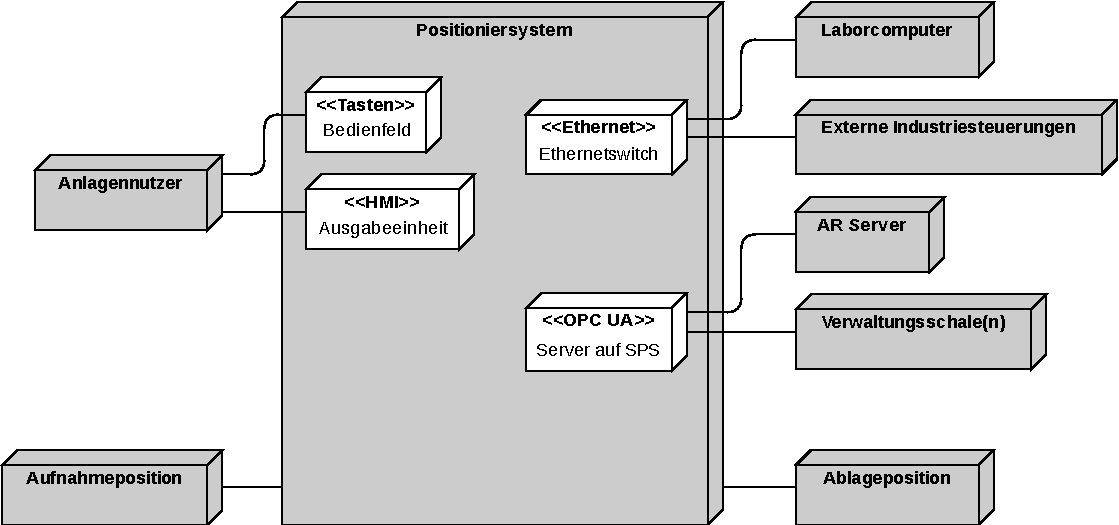
\includegraphics[width=\textwidth]{Images/erster_schritt.pdf}
    \caption[Erster Partitionierungsschritt]{Erster Partitionierungsschritt}
    \label{fig:my-img10}
\end{figure}

\autoref{fig:my-img10} ergänzt zu den bereits bekannten Stereotypen, welche nun in ihren eigenen Knoten aufgeführt werden, die konkreten Knoten als Komponenten des Systems. Wichtig ist hierbei die jeweiligen Anforderungen aus \autoref{anforderungsana} zu den Knoten zu beachten.\\
Die Interaktion des Anlagennutzers mit dem mehrachsigen Positioniersystem erfolgt grundsätzlich über Taster an der SChaltschrankfront der Anlage. Die Menge aller Taster ist im obigen Diagramm zusammengefasst unter dem Begriff Bedienfeld. Auf diesem befinden sich zusätzlich zu den Tastern auch Statusleuchten (Anzeige des ausgewählten Betriebsmodus). Weiterhin ist auch eine Signalampel am äußeren Profil der Laboranlage montiert, wie aus der Beschreibung des Aufbaus der Anlage im \autoref{aufbau} hervorgeht. Sowohl die Leuchten als auch die Ampel fallen nicht unter den Stereotyp Tasten, sondern werden dem allgemeineren Begriff \acf{hmi} zugeordnet. Es handelt sich bei ihnen um anzeigende Elemente. Dementsprechend ist auch der Knotenbegriff Ausgabeeinheit gewählt. \\
Das Wort \textit{Interface} suggeriert jedoch einen Datenaustausch in zwei Richtungen. Das \ac{hmi} im Sinne einer Eingabeeinheit ist in der Industrie meist ein touchfähiges Display, das sowohl Daten Anzeigen kann, als auch Befehle entgegennehmen. Im Fall des Positioniersystems ist solch ein \ac{hmi} in Form eines Tablets oder Smartphones implementiert, welches vom Anlagennutzer entweder selbst mitgebracht wird oder an der Anlage in einer entsprechenden Halterung befestigt ist.\\
Der Knoten Ethernetswitch beschreibt die Schnittstelle zu Nachbarsystemen über das Laborinterne Netzwerk. Dieser wird in der Laboranlage verbaut, um externe Computer und \acsp{sps} mit der Steuerung der Positioniereinheit zu verbinden. Ziel ist es eine Schnittstelle zur verfügung zu stellen, über die von den Laborcomputern das Automatisierungsprogramm auf die Steuerung des Systems gespielt werden kann. \\
Der letzte zu erkennende Knoten, betitelt mit Server auf der \ac{sps}, meint den \ac{opc} UA Server, über welchen Prozessdaten von der Steuerung des Systems (LMC101) bereitgestellt werden. Diese können dann von einem OPC Client, wie \zB dem im Diagramm zu erkennenden \ac{ar} Server entgegengenommen werden, um von diesem anschließend verarbeitet \bzw genutzt zu werden.

\subsubsection{Zweiter Partitionierungsschritt}
Im zweiten Schritt wird die genaue Realisierung der Knoten und der Aufbau des Systems geklärt. Dazu werden die Systemprozessbeschreibungen aus \autoref{AnwfallSpez} benötigt. Ziel ist es das System unter funktionalen Gesichtspunkten in Komponenten \bzw Einheiten zu zerlegen. Dabei wird noch nicht festgelegt, wie die Realisierung der Einheiten mit konkreter Hardware und Software umgesetzt wird. Es findet lediglich eine Aufteilung in funktionale Komponenten statt, welche wiederum in Form von Knoten Symbolisiert werden. \\
\autoref{fig:my-img11} zeigt das entstandene Diagramm nach Anwendung der Systemprozessbeschreibungen auf die im vorherigen Unterabschnitt entwickelte Grafik. 

\begin{figure}[H]
    \centering
    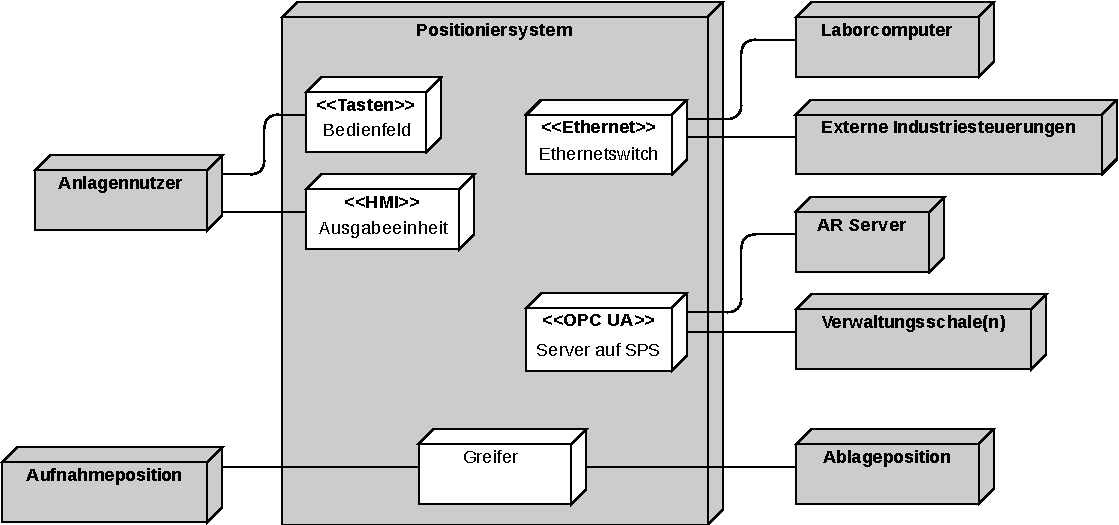
\includegraphics[width=\textwidth]{Images/zweiter_schritt.pdf}
    \caption[Zweiter Partitionierungsschritt]{Zweiter Partitionierungsschritt}
    \label{fig:my-img11}
\end{figure}

Für diesen Partitionierungsschritt sind die \textit{essenziellen Schritte} und die \textit{Kurzbeschreibung} aus unter anderem \autoref{tab:my-table41} relevant. Für die Erstellung der kompletten Grafik müssen alle Anwendungsfallbeschreibungen berücksichtigt werden. Es fällt auf, dass im Vergleich zu Grundlegenden Anwendungsfallbeschreibung im Anwendungsfalldiagramm (\autoref{fig:my-img3}), die Betriebsmodi nicht mit aufgenommen wurden. Grund dafür ist, dass bei der Partitionierung nur die normale Arbeitsweise im Vordergrund steht. Erst bei der Realisierung der in diesem Unterabschnitt gefundenen funktionalen Knoten werden diese wieder betrachtet, da sie eigenschaften dieser Knoten beschreiben.\\
Da zwischen der Aufnahme eines Transportobjektes von der Aufnahmeposition und der Ablage selbigen Objektes auf der Ablageposition nur der Aufnahmeprozess über einen Greifer und der Transportprozess des Positioniersystems selbst stehen, ist im Diagramm nur ein neuer Knoten wiederzufinden. Dieser ist mit dem Begriff \textit{Positioniereinheit} betitelt. Die Positioniereinheit meint an dieser Stelle nicht das gesamte System, sondern ausschließlich die beweglichen Komponenten des Systems (die beiden Achsen mit dem darauf zu montierendem Greifarm inklusive dem Greifer selbst).

\subsubsection{Dritter Partitionierungsschritt}
Im dritten Schritt der Partitionierung findet eine Aufteilung der Komponenten/Einheiten in Software-, Hardware und Anlagenteil statt. Dabei ist die Aufteilung der Einheit unabhängig von der aktuell betrachteten Einheit. Das heißt, soweit es möglich ist, wird die Unterteilung für jede Komponente \bzw Einheit vorgenommen. Existiert eine der drei Unterteilungen nicht für die betrachtete Einheit, entfällt diese.\\
Die \autoref{fig:my-img12} zeigt die prinzipielle Aufteilung der einzelnen Einheiten des Systems.

\begin{figure}[H]
    \centering
    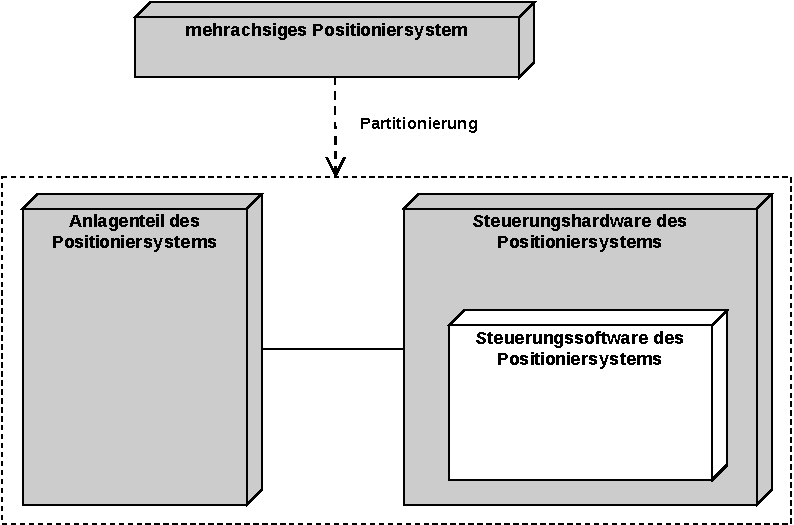
\includegraphics[width=0.8\textwidth]{Images/dritter_schritt.pdf}
    \caption[Dritter Partitionierungsschritt]{Dritter Partitionierungsschritt - Aufteilungsprinzip}
    \label{fig:my-img12}
\end{figure}

Es ist zu erkennen, dass die Grafik aus drei Knoten besteht, die genau die drei Teile Anlage, Hardware und Software darstellen. Gemeinsam decken sie die Funktionalität einer Einheit ab. Ausgehend von dieser Darstellung werden nachfolgend die Schnittstellen und prinzipiellen Eigenschaften dieser Knoten entwickelt und in einer Knotenbeschreibung dokumentiert. \\ % (siehe Tabelle) verlinkung hinzufügen
In diesem Schritt treten die nicht funktionalen Anforderungen an das System wieder in den Vordergrund. Aufgabe ist es nun die Anforderungen nach Informationen an das Design des Systems zu durchleuchten. Ziel ist es zu jeder der drei erwähnten Unterteilungen spezifische Umsetzungen zu finden \bzw zu entwickeln, falls aus den \acp{nfa} keine Designentscheidungen entnehmbar sind. \\
Konkret das mehrachsige Positioniersystem betreffend ist aus den Anforderungen zu erkennen, das für die Steuerungshardware der Positioniereinheit ein \ac{lmc} von Schneider Electric vorgesehen ist, und für die Energiemessung eine Wago \ac{sps} der PFC200 Serie. Zur Steuerungshardware zugehörig sind weiterhin sowohl das Netzteil und der Servoregler. Beide werden in den Anforderungen bereits erwähnt. Es steht fest, um welche Modelle es sich handelt (\acs{lxm}62 Serie).\\ 
Auch zu den Aktuatoren und Sensoren der Steuerungshardware werden Aussagen in der Anforderungsanalyse getroffen. Für die Endlagendetektierung werden induktive Näherungsschalter verwendet. Der Lichtvorhang zum SChutz für Leib und Leben wird auch als Sensor kategorisiert und ist bereits ausgewählt (XUS Serie von Schneider Electric). Bei den Aktuatoren des Systems handelt es sich um multiturn Servos aus der Produktserie SH3 (ebenfalls von Schneider Electric). \\
Der generelle Aufbau des Systems bestehend aus Gehäuse und Schaltschrank wird nicht direkt in den Anforderungen vorgegeben. Somit müssen erst Anforderungen für den ANlagenteil des Systems getroffen werden. Für die Entscheidung zur Wahl der konkreten Profile, aus denen das Gehäuse aufgebaut wird, sowie die beweglichen Schlitten auf den beiden Achsen und der Schaltschrank, sollten Fachleute herangezogen werden. Im Falle der Laboranlage wurden Designentscheidungen aus den nicht funktionalen Anforderungen des Laboringenieurs Dipl. Ing. Dirk Schöttke (wiederzufinden in der Stakeholdertabelle) getroffen. Es handelt sich dabei hauptsächlich aus Erfahrungen mit bereits umgesetzten Systemen. Resultat ist die Wahl von Profilen und beweglichen Schlitten der Firma MiniTec. Auch die Entscheidung, welcher Schaltschranke ausgewählt wird, wird Anhand der definierten \acp{nfa} von Herr Schöttke getroffen. Zu beachten ist, dass der Schaltschrank genügend Platz für alle benötigten Komponenten bereitstellt.\\
Noch zu Untersuchen sind die Anforderungen nach Designinformationen zur Steuerungssoftware des Positioniersystems. Aus den nicht funktionalen Anforderungen an die Steuerungshardware erübrigt sich die Wahl der Steuerungssoftware des Positioniersystems. Durch die Nutzung des Logic Motion Controllers von Schneider Electric ist die Programmierung dieses eingeschränkt auf die Entwicklungsumgebung, die ebenfalls durch Schneider Electric bereitgestellt wird. Die später auf der Laboranlage ausgeführte Automatisierungssoftware muss in der SoMachine \bzw MachineExpert Entwicklungsumgebung generiert werden, um diese auf der Steuerung des Systems nutzen zu können. Es handelt sich folglich um ein abgeschlossenes Ökosystem, welches vom Hersteller etabliert wurde. Resultat ist somit auch eine vorgeschriebene Vorgehensweise zur Umsetzung von Motion Software für das Positioniersystem. Die Steuerungssoftware der PFC200 \ac{sps} soll an dieser Stelle nicht unerwähnt bleiben. Die konfiguration der STeuerung bedingt die Nutzung der Software e!Cockpit von Wago zur Programmierung der Steuerungssoftware für die Energiemessungskomponente des Systems.\\
Nachdem alle Partitionierungsentscheidungen bezüglich der Anlage getroffen wurden, werden diese in Form einer Tabelle dokumentiert. Dabei handelt es sich um die Beschreibung der Knoten aus dem Verteilungsdiagramm in \autoref{fig:my-img12}.\\
Die erste Tabelle (\autoref{tab:my-table50}) behandelt den Anlagenteil der Positioniereinheit. Die Felder der Tabelle enthalten alle wichtigen Informationen über den Knoten des Anlagenteils der Positioniereinheit. Zu dokumentieren sind die Informnationen \textbf{Name}, \textbf{Typ}, \textbf{Beschreibung}, \textbf{\acp{fa}} und \textbf{\acp{nfa}}. Im Eintrag \textit{Typ} wird die Knotenart definiert, also ob es sich um Software, Hardware oder die Anlage handelt. Die funktionalen und nicht funktionalen Anforderungen, die sich auf den Knoten beziehen weren ebenfalls in der Tabelle aufgenommen.

\begin{table}[H]
    \centering
    \begin{tabular}{| p{0.34\linewidth} | p{0.6\linewidth} |}
        \hline
        \textbf{Name} & Anlagenteil des Positioniereinheit \\ \hline
        \textbf{Typ} & Anlage \\ \hline
        \textbf{Beschreibung} & Stellt die Infrastruktur bereit, an die die Aktuatoren und Sensoren der Steuerungshardware angeschlossen sind. \\ \hline
        \textbf{Funktionale Anforderungen} & Die Anlage muss sich entlang der horizontalen und vertikalen Achse bewegen können und wieder abbremsen. Weiterhin muss sie über einen Greifarm/Greifer Kombination Transportgüter aufnehmen und wieder ablegen können. \\ \hline
        \textbf{Nicht funktionale Anforderungen} & Die Anlage muss in den Laborraum G422 integriert werden. Zur sicherheit sollen Plexiglasabdeckungen an ungeschützten Bereichen montiert werden. Kabel sollen in E-Ketten an den beweglichen Achsen mitgeführt werden. \\ \hline
    \end{tabular}
    \caption[Knotenpunktbeschreibung - Anlagenteil]{Knotenpunktbeschreibung der Positioniereinheit - Anlagenteil}
    \label{tab:my-table50}
\end{table}

Analog zur ersten Tabelle wird anschließend die Knotenbeschreibung zur Hardware und Software der Positioniereinheit vorgenommen.

\begin{table}[H]
    \centering
    \begin{tabular}{| p{0.34\linewidth} | p{0.6\linewidth} |}
        \hline
        \textbf{Name} & Steuerungshardware des Positioniereinheit \\ \hline
        \textbf{Typ} & Hardware \\ \hline
        \textbf{Beschreibung} & Die Hardware besteht aus den Controllern (LMC und PFC200), Aktuatoren und Sensoren. Diese sind zur Erfüllung der Aufgaben der Positioniereinheit nötig. \\ \hline
        \textbf{Funktionale Anforderungen} & Die Servomotoren der Achsen sollen über den LMC gesteuert Positionieraufgaben ausführen. Dafür wird eine Powersupply/Servoregler Kombination benötigt, um die Motoren zu betreiben. Über Endlagesensoren soll verhindert werden, dass Bewegungen über die Enden der beiden Achsen hinaus durchgeführt werden können. Mit Hilfe eines zweiten Controllers soll die Energiezufuhr zum gesamten System gemessen werden. Nutzereingaben sollen über ein Bedienfeld an der Schaltschrankfront und/oder über ein Display erfolgen. Zur Signalisierung von Gefahrensituationen ist eine Signalampel zu verbauen. \\ \hline
        \textbf{Nicht funktionale Anforderungen} & Die Steuerungshardware der Positioniereinheit stammt aus der PacDrive3 Reihe von Schneider Electric. Erweitert wird diese um zwei Motoren und einen Lichtvorhang, die ebenfalls von Schneider Electric gestellt werden. Um weitere digitale und Anlago (sichere) Ausgänge beritzustellen, sollen Module aus der TM5 Serie von Schneider Electric im Schaltschrank verbaut werden. Die SPS für die Energiemessung ist ein PFC200 Controller von Wago. \\ \hline
    \end{tabular}
    \caption[Knotenpunktbeschreibung - Hardware]{Knotenpunktbeschreibung der Positioniereinheit - Hardware}
    \label{tab:my-table51}
\end{table}

Durch die Vorhgabe der Steuerungssoftware stehen die Schnittstellen zwischen den Steuerkomponenten und den Sensoren sowie Aktuatoren bereits fest. Der LMC400 kommuniziert mit den TM5 Erweiterungsmodulen, dem LXM62 P (Powersupply) und LXM62 D (Servoregler) via SercosIII (in Ringkonfiguration). Zu den Endlagesensoren führen dreiadrige Sensorleitungen. Der Lichtvorhang (bestehend aus Emitter und Receiver) ist ebenfalls über 8 und 11 adrige Sensorleitungen am Controller (über Klemmen im Schaltschrank) angeschlossen. Zu den beiden Motoren führt sowohl ein Stromkabel (3-phasig) und eine Encoderkabel (für die Bremsfunktion und das Auslesen von \zB Temperaturwerten). Die beiden Cotroller sind unternander und auch mit allen weiteren Computern im Labornetzwerk per Ethernet über einen im Schaltschrank verbauten Switch verbunden.

\begin{table}[H]
    \centering
    \begin{tabular}{| p{0.34\linewidth} | p{0.6\linewidth} |}
        \hline
        \textbf{Name} & Steuerungssoftware der Positioniereinheit \\ \hline
        \textbf{Typ} & Software \\ \hline
        \textbf{Beschreibung} & Die Steuerungssoftware wertet Sensordaten aus, berechnet Trajektorien und Geschwindigkeiten für die Achsenpositionierung und stellt Prozessdaten aus globalen Variablenlisten bereit.  \\ \hline
        \textbf{Funktionale Anforderungen} & Berechnet Fahrtwege, Geschwindigkeiten und Beschleunigungen aus Nutzereingaben \bzw Vorgaben. Weiterhin wird für das sicherheitsgerechte Bremsen bei Erreichen von Endlagen oder der Not-Halt-Auslösung gesorgt.  \\ \hline
        \textbf{Nicht funktionale Anforderungen} & Die Automatisierungssoftware muss in der LogicBuilder Entwicklungsumgebung erstellt werden. Diese Umgebung wird bereits mit einigen Entwicklungsvorgehensweisen \bzw Routinen ausgeliefert. \\ \hline
    \end{tabular}
    \caption[Knotenpunktbeschreibung - Software]{Knotenpunktbeschreibung der Positioniereinheit - Software}
    \label{tab:my-table52}
\end{table}

Da das Positioniersystem nur aus einer Einheit, der Positioniereinheit besteht, kann der dritte Partitionierungsschritt mit drei Tabellen (Anlage, Software, Hardware) modelliert werden. Die weniger hohe Komplexität (bedingt durch das Nichtvorhandensein von mehreren Untereinheiten) führt zu der Partitionierung in die Grundlegenden Einheiten \textit{Anlagenteil}, \textit{Steuerungshardware} und \textit{Steuerungssoftware} der Positioniereinheit.\\
Auf Basis der Partitionierung kann in der Anlagenprojektierung nun die Entwicklung der Systemsoftware durchgeführt werden, nachdem die detaillierte Systemanalyse mit diesem Unterabschnitt beendet ist. Wie bereits eingangs erwähnt, folgt zunächst die Dokumentation der Testspezifikation, welche nach der Projektierung für die Inbetriebnahme der in der Projektierung entwickelten Software benötigt wird.

\end{document}